\documentclass{article}
\usepackage{cmap}
\usepackage[utf8]{inputenc}
\usepackage[english,ukrainian]{babel}
\usepackage{graphicx}
\usepackage{geometry}
\usepackage{listings}
\usepackage{indentfirst}
\usepackage{subfigure}
\usepackage{caption}
\usepackage{amsmath}
\geometry{
	a4paper,
	left=20mm,
	right=20mm,
	top=20mm,
	bottom=20mm
}
\lstset{
	extendedchars=\true,
	tabsize=4,
	language=python,
	showstringspaces=false,
	showtabs=false,
	frame=lrtb,
	columns=fixed,
	keepspaces,
	breaklines=true
}
\graphicspath{ {pictures} }
\setlength{\parindent}{4em}
\newcommand\subject{Чисельні методи ПЗ}
\newcommand\lecturer{доцент кафедри ПЗ\\Мельник Н.Б.}
\newcommand\teacher{асистент кафедри ПЗ\\Гарматій Г.Ю.}
\newcommand\mygroup{ПЗ-16}
\newcommand\lab{4}
\newcommand\theme{Розв’язування систем лінійних алгебраїчних рівнянь методом Гауса та методом LU-розкладу}
\newcommand\purpose{Ознайомлення на практиці з методом Гауса та методом LU-
	розкладу розв’язування систем лінійних алгебраїчних рівнянь}

\begin{document}
	\begin{large}
		\begin{titlepage}
			\thispagestyle{empty}
			\begin{center}
				\textbf{МІНІСТЕРСТВО ОСВІТИ І НАУКИ УКРАЇНИ\\
					НАЦІОНАЛЬНИЙ УНІВЕРСИТЕТ "ЛЬВІВСЬКА ПОЛІТЕХНІКА"}
			\end{center}
			\begin{flushright}
				Інститут \textbf{КНІТ}\\
				Кафедра \textbf{ПЗ}
			\end{flushright}
			\vspace{200pt}
			\begin{center}
				\textbf{ЗВІТ}\\
				\vspace{10pt}
				До лабораторної роботи № \lab\\
				\textbf{На тему}: “\textit{\theme}”\\
				\textbf{З дисципліни}: “\subject”
			\end{center}
			\vspace{90pt}
			\begin{flushright}
				
				\textbf{Лектор}:\\
				\lecturer\\
				\vspace{28pt}
				\textbf{Виконав}:\\
				
				студент групи \mygroup\\
				Коваленко Д.М.\\
				\vspace{28pt}
				\textbf{Прийняла}:\\
				
				\teacher\\
				
				\vspace{28pt}
				«\rule{1cm}{0.15mm}» \rule{1.5cm}{0.15mm} 2022 р.\\
				$\sum$ = \rule{1cm}{0.15mm}……………\\
				
			\end{flushright}
			\vspace{\fill}
			\begin{center}
				\textbf{Львів — 2022}
			\end{center}
		\end{titlepage}
		
		\begin{description}
			\item[Тема.] \theme.
			\item[Мета.] \purpose.
		\end{description}
		
		\section*{Теоретичні відомості}
		\subsection*{Метод Гауса}
		Суть методу Гауса полягає в тому, що систему лінійних алгебраїчних рівнянь зводять до
		еквівалентної системи з верхньою (або нижньою) трикутною матрицею.
		Невідомі знаходять послідовними підстановками, починаючи з останнього
		рівняння перетвореної системи.
		\begin{gather}
			\left\{\begin{array}{@{}l@{}}
				a_{11}x_1 + a_{12}x_2 + ... + a_{1n}x_n = b_{1},\\\nonumber
				a_{21}x_1 + a_{22}x_2 + ... + a_{2n}x_n = b_{2},\\\nonumber
				.................................................\\\nonumber
				a_{n1}x_1 + a_{n2}x_2 + ... + a_{nn}x_n = b_{n}.\nonumber
			\end{array}\right.\,\\
			\left\{\begin{array}{@{}l@{}}
				a_{11}x_1 + a_{12}x_2 + ... + a_{1n}x_n = b_{1},\\\nonumber
				0x_1 + a_{22}x_2 + ... + a_{2n}x_n = b_{2},\\\nonumber
				.................................................\\\nonumber
				0x_1 + 0x_2 + ... + a_{nn}x_n = b_{n}.\nonumber
			\end{array}\right.\,\\
		x_n=\frac{b_n^{n-1}}{a_{nn}^{(n-1)}}\nonumber
		\end{gather}
		\subsection*{Метод LU-розкладу}
		Метод LU-розкладу полягає в розкладі матриці $A$ коефіцієнтів системи на добуток двох матриць –
		нижньої трикутної матриці $L$, елементи головної діагоналі якої не дорівнюють
		нулеві та верхньої трикутної $U$, на головній діагоналі якої містяться одиниці,
		тобто
		\begin{gather}
			A=LU\nonumber,
		\end{gather}
		де
		\begin{gather}\nonumber
			L=\begin{pmatrix}
				l_{11} & 0 & 0 & ... & 0\\
				l_{21} & l_{22} & 0 & ... & 0\\
				l_{31} & l_{32} & l_{33} & ... & 0\\
				... & ... & ... & ... & ...\\
				l_{n1} & l_{n2} & l_{n3} & ... & l_{nn}
			\end{pmatrix}
			\hspace{28pt}
			U=\begin{pmatrix}
				1 & u_{12} & u_{13} & ... & u_{1n}\\
				0 & 1 & u_{23} & ... & u_{2n}\\
				0 & 0 & 1 & ... & u_{3n}\\
				... & ... & ... & ... & ...\\
				0 & 0 & 0 & ... & 1
			\end{pmatrix}\nonumber
		\end{gather}
	
		Увівши допоміжний вектор $Y$, такий, що $UX=Y$.
		Тоді матричне рівняння подамо у вигляді $LY=B$.
		
		Отримуємо компоненти вектора $Y$
		\begin{gather}
			y_i=\frac{1}{l_{ii}}(b_i-\sum_{m=1}^{i-1}l_{im}y_m), \hspace{28pt} i=\overline{2,n}\nonumber
		\end{gather}
	
		Далі послідовно знаходимо компоненти
		вектора $X$
		\begin{gather}
			x_n=y_n\hspace{28pt}x_i=y_i-\sum_{m=i+1}^{n}u_{im}x_m,\hspace{28pt}i<n\nonumber
		\end{gather}
	
		\section*{Лабораторне завдання}
		\begin{enumerate}
			\item Ознайомитись з теоретичними відомостями.
			\item Скласти програму розв’язування системи лінійних алгебраїчних рівнянь
			методом Гауса та методом LU-розкладу.
			\begin{gather}\nonumber
				\left\{\begin{array}{@{}l@{}}
					0.34x_1 + 0.71x_2 + 0.63x_3 = 2.08\\\nonumber
					0.71x_1 - 0.65x_2 - 0.18x_3 = 0.17\\\nonumber
					1.17x_1 - 2.35x_2 + 0.75x_3 = 1.28\nonumber
				\end{array}\right.\,
			\end{gather}
		\end{enumerate}
	
		\section*{Хід роботи}
		\subsection*{Метод Гауса}
		\begin{gather}\nonumber
		\left\{\begin{array}{@{}l@{}}
			0.34x_1 + 0.71x_2 + 0.63x_3 = 2.08\\\nonumber
			0.71x_1 - 0.65x_2 - 0.18x_3 = 0.17\\\nonumber
			1.17x_1 - 2.35x_2 + 0.75x_3 = 1.28\nonumber
		\end{array}\right.\,\\
		\left\{\begin{array}{@{}l@{}}
			0.34x_1 + 2.08x_2 + 1.85x_3 = 6.11\\\nonumber
			\hspace{38pt} - 0.83x_2 - 1.13x_3 = -4.17\\\nonumber
			\hspace{38pt} - 0.09x_2 - 1.41x_3 = -5.87\nonumber
		\end{array}\right.\,\\
		\left\{\begin{array}{@{}l@{}}
			0.34x_1 \hspace{41pt} -0.33x_3 = -1.47\\\nonumber
			\hspace{32pt} -0.83x_2 -1.13x_3 = -4.17\\\nonumber
			\hspace{80pt}- 1.29x_3 = -5.41\nonumber
		\end{array}\right.\,\\
		\left\{\begin{array}{@{}l@{}}
			0.34x_1 \hspace{88pt} = -1.47\\\nonumber
			\hspace{39pt} -0.83x_2 \hspace{40pt} = -4.17\\\nonumber
			\hspace{80pt} -1.29x_3 = -5.41\nonumber
		\end{array}\right.\,\\
		\left\{\begin{array}{@{}l@{}}
			x_1 = -1.17\\\nonumber
			x_2 = -0.70\\\nonumber
			x_3 = 4.19\nonumber
		\end{array}\right.\,
		\end{gather}	
		\noindent\textit{\textbf{Код програми} (файл lab\_\lab1.py):}
		\begin{lstlisting}
import numpy as np

def gauss_method(A, n):
	""" Метод Гауса """
	print(gauss_method.__doc__)
	for i in range(n):
		if A[i][i] == 0.0: 
			exit("Помилка: елемент головної діагоналі = 0")
		for j in range(n):
			if i != j:
				ratio = A[j][i]/A[i][i]
				for k in range(n + 1):
					A[j][k] -= ratio * A[i][k]
	print("Відповідь: ",[round(A[i][n]/A[i][i],4) for i in range(n)])

path = input("Введіть шлях до файлу з даними: ") or "data.csv"
A = np.loadtxt(open(path, "rb"), delimiter=",")
gauss_method(A, np.shape(A)[0])\end{lstlisting}
		
		\subsection*{Метод LU-розкладу}
		\begin{gather}\nonumber
		A=LU\\\nonumber
		\begin{pmatrix}
			0.34 & 0.71 & 0.63\\
			0.71 & 0.65 & 0.18\\
			1.17 & 2.35 & 0.75
		\end{pmatrix}
	=
		\begin{pmatrix}
			l_{11} & 0 & 0\\
			l_{21} & l_{22} & 0\\
			l_{31} & l_{32} & l_{33}
		\end{pmatrix}
		\begin{pmatrix}
			1 & u_{12} & u_{13}\\
			0 & 1 & u_{23}\\
			0 & 0 & 1
		\end{pmatrix}\\\nonumber
		\begin{pmatrix}
			0.34 & 0.71 & 0.63\\
			0.71 & 0.65 & 0.18\\
			1.17 & 2.35 & 0.75
		\end{pmatrix}
	=
		\begin{pmatrix}
			l_{11} & l_{11}u_{12} & l_{11}u_{13}\\
			l_{21} & l_{21}u_{12}+l_{22} & l_{21}u_{13}+l_{22}u_{23}\\
			l_{31} & l_{31}u_{12}+l_{32} & l_{31}u_{13}+l_{32}u_{23}+l_{33}
		\end{pmatrix}\\\nonumber
		ll_{11}=0.34\\\nonumber
		l_{11}u_{12}=0.71 \Rightarrow 0.34u_{12}=0.71 \Rightarrow u_{12}=2.08\\\nonumber
		l_{11}u_{13}=0.63 \Rightarrow 0.34u_{13}=0.63 \Rightarrow u_{13}=1.85\\\nonumber
		L=\begin{pmatrix}
			0.34 & 0 & 0\\
			0.71 & -0.83 & 0\\
			1.17 & -0.09 & -1.29
		\end{pmatrix}\\\nonumber
		U=\begin{pmatrix}
			1 & 2.08 & 1.85\\
			0 & 1 & 1.36\\
			0 & 0 & 1
		\end{pmatrix}\\\nonumber
		LY=B,\hspace{28pt}Y=L^{-1}B\\\nonumber
		Y=\begin{pmatrix}
			6.11 & 5.01 & 4.19
		\end{pmatrix}\\\nonumber
		UX=Y,\hspace{28pt}X=U^{-1}Y\\\nonumber
		X=\begin{pmatrix}
			-1.17 & -0.70 & 4.19
		\end{pmatrix}
		\end{gather}
		\noindent\textit{\textbf{Код програми} (файл lab\_\lab2.py):}
		\begin{lstlisting}
import numpy as np

def data_to_matrix(path):
	return (
		np.loadtxt(open(path,"rb"), delimiter=",", usecols=[0,1,2]),
		np.loadtxt(open(path,"rb"), delimiter=",", usecols=3),
	)

def invert_matrix(A, n):
	A_1 = np.array(A)
	for i in range(n):
		for j in range(n):
			tmp = np.delete(A, i, 0)
			tmp = np.delete(tmp, j, 1)
			A_1[i][j] = (-1)**((i) + (j)) * np.linalg.det(tmp) / np.linalg.det(A)
	return np.transpose(A_1)

def lu_decomposition_method(A, B, n):
	""" Метод LU-розкладу """
	print(lu_decomposition_method.__doc__)
	L = [[0] * n for i in range(n)]
	U = [[0] * n for i in range(n)]
	for j in range(n):
		U[j][j] = 1
		for i in range(j, n):
			alpha = A[i][j]
			for k in range(j):
				alpha -= L[i][k]*U[k][j]
			L[i][j] = alpha
		for i in range(j+1, n):
			tempU = A[j][i]
			for k in range(j):
				tempU -= L[j][k]*U[k][i]
			U[j][i] = tempU/L[j][j]
	Y = np.matmul(invert_matrix(L, n), B) # Обчислюємо Y
	X = np.matmul(invert_matrix(U, n), Y) # Обчислюємо X
	print("Відповідь:", [round(x, 4) for x in X])

path = input("Введіть шлях до файлу з даними: ") or "data.csv"
A, B = data_to_matrix(path)
lu_decomposition_method(A, B, np.shape(A)[0])\end{lstlisting}
		
		\begin{figure}[h!]
			\centering
			\subfigure[]{\includegraphics[width=0.5\textwidth]{1}}\\
			\subfigure[]{\includegraphics[width=0.5\textwidth]{2}}\\
			\subfigure[]{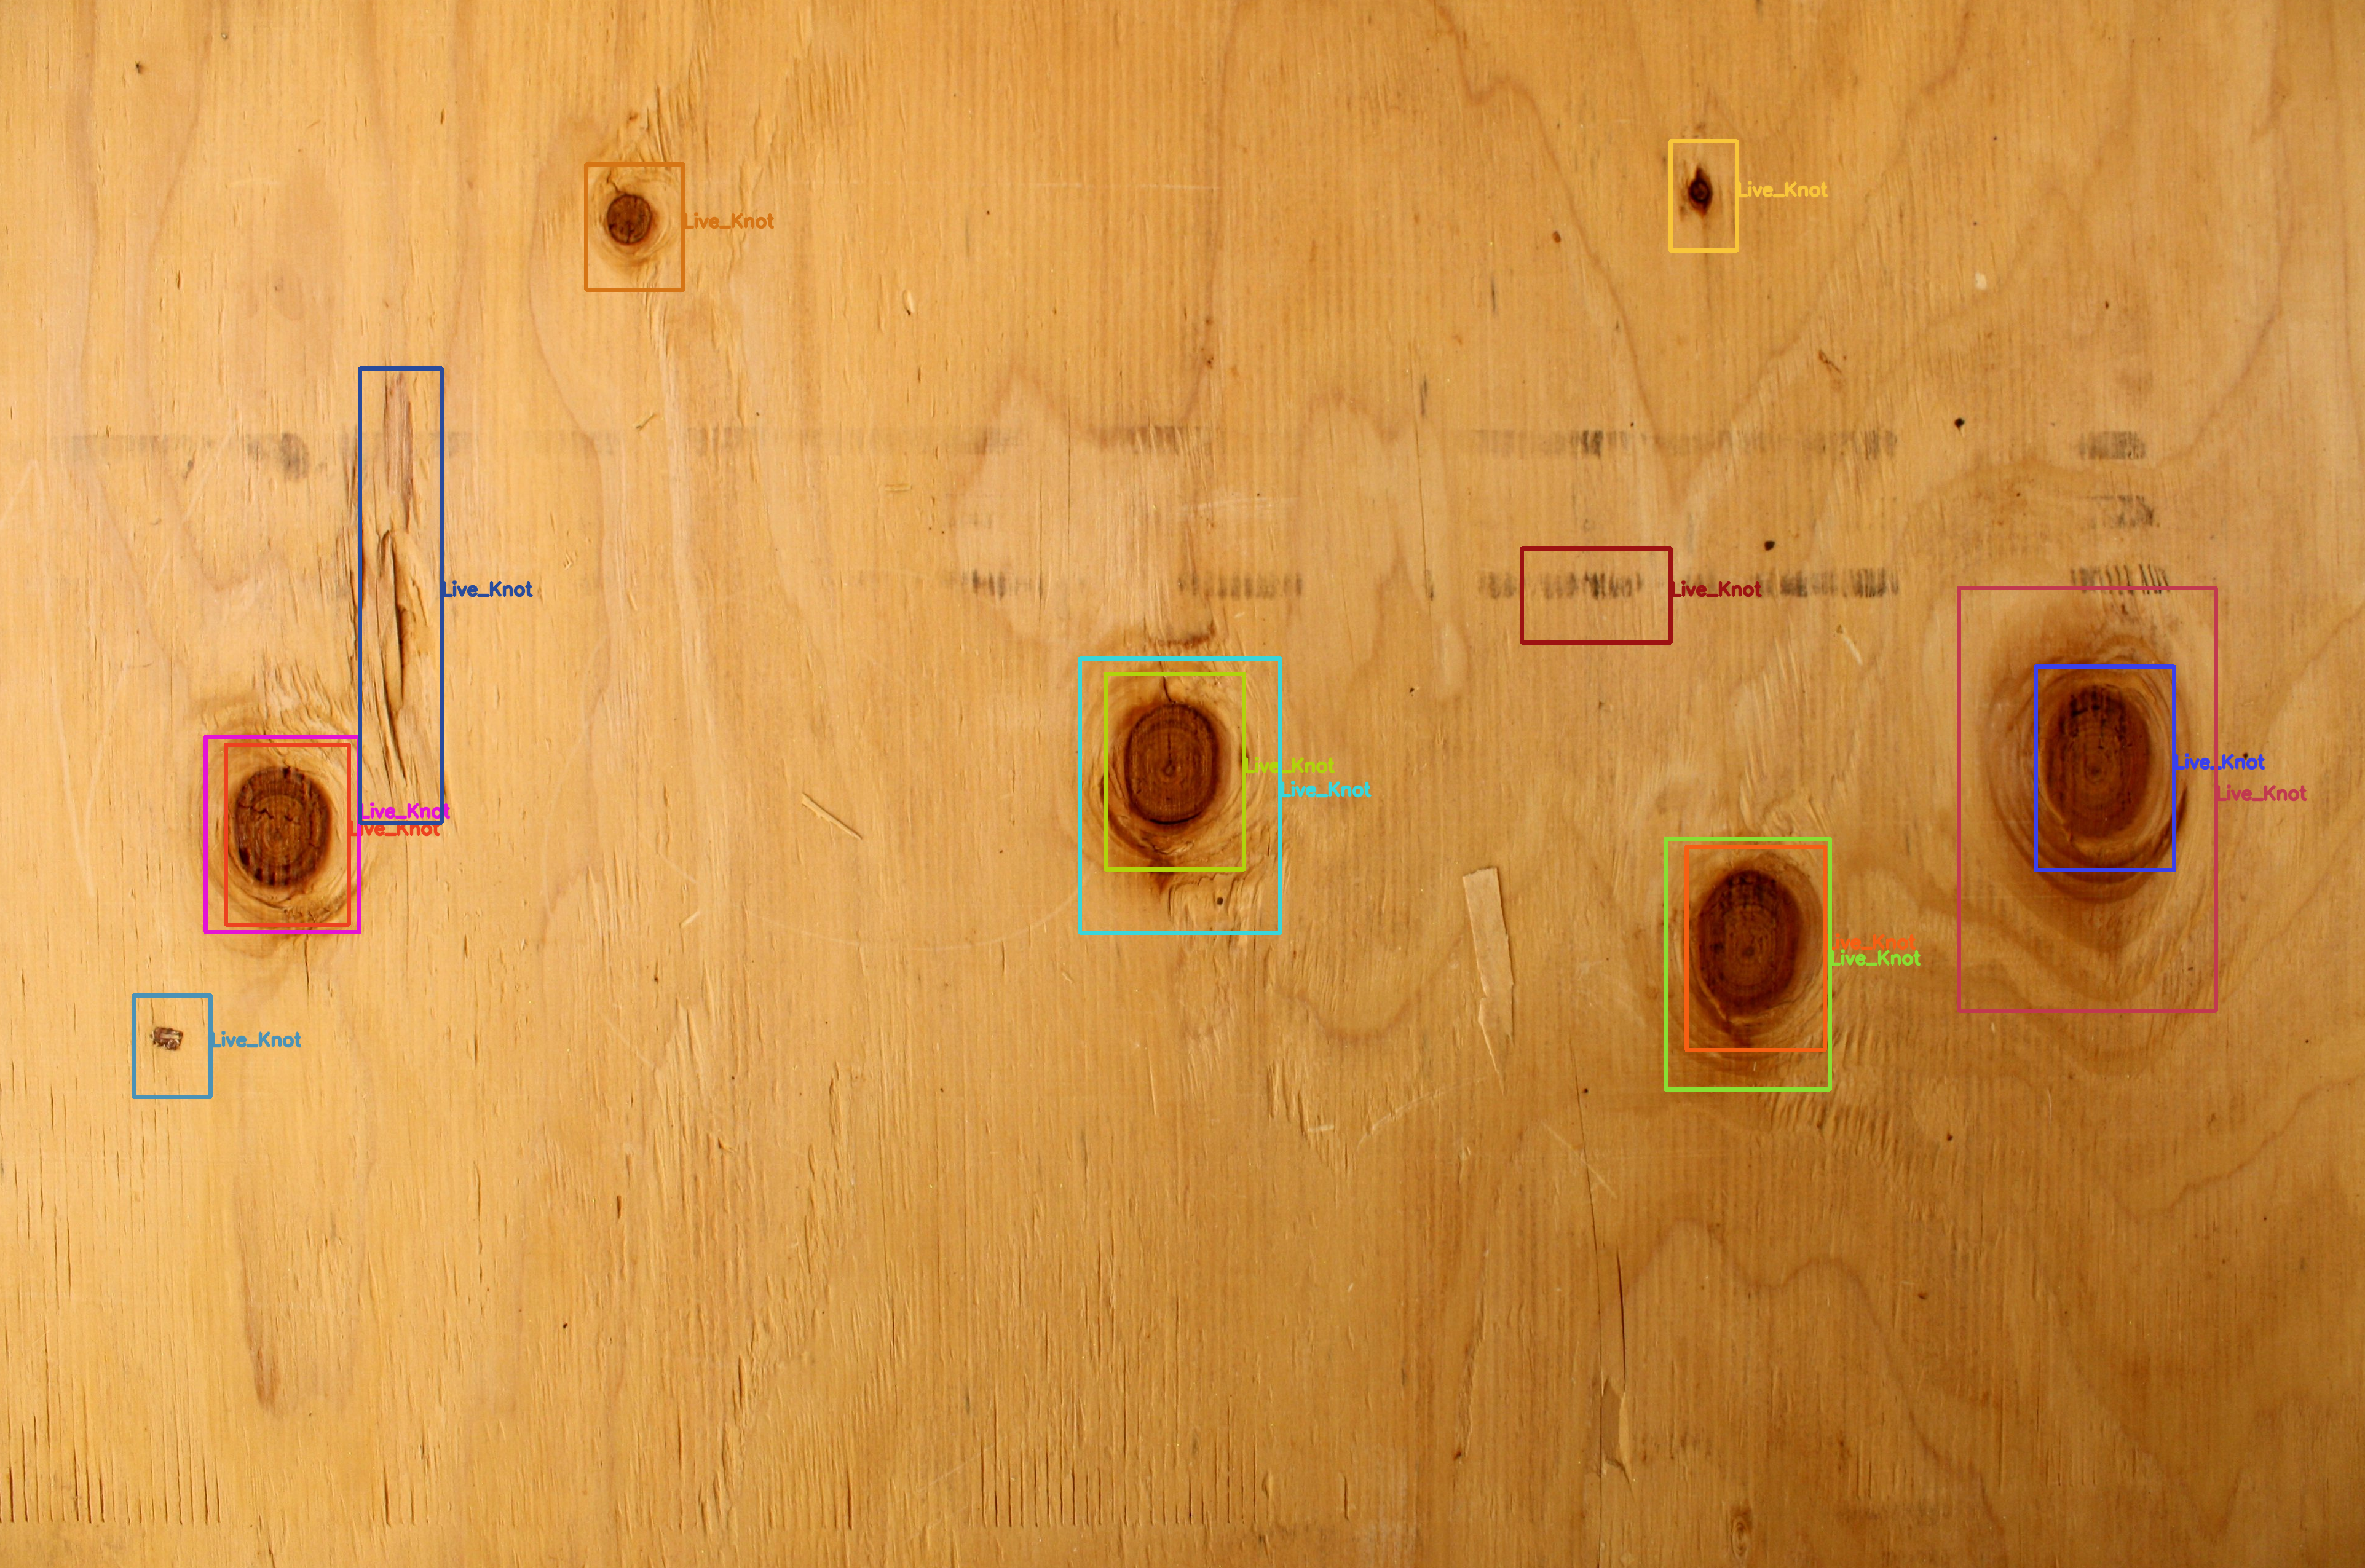
\includegraphics[width=0.4\textwidth]{3}}
			\caption{Метод Гауса (а), метод LU-розкладу (б), файл даних (в)}
		\end{figure}
		
		\section*{Висновок}
		На лабораторній роботі я засвоїв практичні навички використання методу Гауса та методу LU-розкладу та розробив функції для розв’язку системи лінійних алгебраїчних рівнянь 
		\begin{gather}\nonumber
			\left\{\begin{array}{@{}l@{}}
				0.34x_1 + 0.71x_2 + 0.63x_3 = 2.08\\\nonumber
				0.71x_1 - 0.65x_2 - 0.18x_3 = 0.17\\\nonumber
				1.17x_1 - 2.35x_2 + 0.75x_3 = 1.28\nonumber
			\end{array}\right.\,
		\end{gather}
		за допомогою цих методів. Корені системи рівнянь: $-1.1786; -0.7041; 4.1915$.
		
	\end{large}
\end{document}
